\begin{filecontents}{leer.eps}
%!PS-Adobe-2.0 EPSF-2.0
%%CreationDate: Mon Jul 13 16:51:17 1992
%%DocumentFonts: (atend)
%%Pages: 0 1
%%BoundingBox: 72 31 601 342
%%EndComments

gsave
72 31 moveto
72 342 lineto
601 342 lineto
601 31 lineto
72 31 lineto
showpage
grestore
%%Trailer
%%DocumentFonts: Helvetica
\end{filecontents}
%
\documentclass[epj]{svjour}
% Remove option referee for final version
%
% Remove any % below to load the required packages
%\usepackage{latexsym}
%\usepackage{graphics}
\usepackage{graphicx}
\usepackage{epstopdf}
% etc
%
\begin{document}
%
\title{Network analysis of metabolic subsystems}
%\subtitle{Do you have a subtitle?\\ If so, write it here}
\author{Rok Novosel\thanks{\email{rn0450@student.uni-lj.si}} \and Matija
  \v{C}ufar\thanks{\email{matijacufar@gmail.com}}
% \thanks is optional - remove next line if not needed
%\thanks{\emph{Present address:} Insert the address here if needed}%
}                     % Do not remove
%
\institute{Faculty of Computer and Information Science}
%
%\date{Received: date / Revised version: date}
%
\abstract{Subsystems are parts of a metabolism that perform different important
  tasks in a cell. In this article, we explore these subsystems from a network
  science point of view. We attempt to find ways of detecting subsystems in a
  metabolic network using community detection algorithms. We use the Louvain modularity
  optimization algorithm as a baseline against which we compare the effectiveness of other
  algorithms. We use the Girvan-Newman algorithm and a novel approach using higher order structures for
  network clustering as a comparison.
  We use the algorithms on a metabolic network of the Chinese hamster ovary cell, a mammalian cell
  that is commonly used in biomedical research and in biotechnology.}

% tole gre v abstract
%\PACS{
%      {PACS-key}{discribing text of that key}   \and
%      {PACS-key}{discribing text of that key}
%     } % end of PACS codes

\maketitle

\section{Introduction}
\label{sec:intro}

Since the turn of the century, life sciences have been evolving
rapidly. Advances in data acquisition, storage and analysis technology have
allowed scientist to gather immense amounts of data and build complex models
from it~\cite{modsys}. These complicated models have brought people of various
backgrounds, such as physics, mathematics and computer science into the field
of biology.

One such field is network science, which
is often used to analyze different kinds of networks that appear in the various
subfields of modern biology, including ecology~\cite{proulx2005network}, systems
biology~\cite{barabasi2004network} and neuroscience~\cite{sporns2014contributions}.

Metabolic networks~\cite{jeong2000large} are used to model the meta-bolisms of
various organisms. They are usually represented with a bipartite graph composed
of two types of vertices: reactions and chemicals produced and consumed by the
reactions. The edges in such a network connect chemicals to
reactions. Furthermore, the edges are directed indicating whether the chemical
was produced or consumed. A third kind of vertex can be added to represent
enzymes that catalyze the reaction, but do not directly partake in
it. Other commonly used representations are simplified representations, where
one of the types of vertices is omitted~\cite{newman2010networks}.

In this article, we analyze the subsystems in a metabolic network of the
Chinese hamster ovary cell. We explore different methods of detecting the
subsystems and compare their structures.

\section{Related works}
% benson2016higher - motifs
% jeong2000large - scale free
% holme2003subnetwork

Paper~\cite{jeong2000large} offers a general overview of the organization and structure of metabolic networks. 
They compare the metabolic networks of 43 different organisms and find that
metabolic networks belong to the class of scale-free networks. Moreover, they find that the network diameter is
consistent across all of the analyzed networks. 

In~\cite{holme2003subnetwork} they present a method to decompose metabolic networks into subnetworks based on the global network structure. They use a modified Girvan-Newman algorithm~\cite{girvan2002community} to construct a hierarchical clustering tree. They argue that instead of looking at a particular partitioning of a network, we should look at the hierarchical clustering tree as whole, since well-defined subnetworks appear at different heights.

A framework for clustering networks based on higher order structures (e.g. motifs) is introduced in~\cite{benson2016higher}.

\section{Methods}
\label{sec:methods}

We apply a few different community detection methods and compare how well
they detect the subsystems of a metabolic network.

We haven't decided on the algorithms yet, but we try some of the following:

\begin{itemize}
\item
  Some of the algorithms from the lectures.
\item
  Community detection based on motifs~\cite{benson2016higher}.
\item
  Removing nodes with the highest betweenness centrality (or some other measure)
  and observing how the network falls apart~\cite{holme2003subnetwork}.
\end{itemize}

\section{Results}
\label{sec:results}

In this article, we analyse a metabolic network of the Chinese hamster
ovary (CHO) cell. The CHO cell is frequently used in biological and medical
research and in the production of biopharmaceuticals~\cite{chocons}.

We used a whole-cell metabolic network of the Chinese hamster ovary (CHO)
cell that was taken from the BiGG database~\cite{bigg,chocons}. The original
network contains 4,456 metabolites that take part in 6,663 reactions. The
reactions and metabolites are annotated with additional metadata, such as name,
subsystem, BiGG ID etc.

We simplify the network to a simple directed graph, where reactions are
represented with nodes. If one reaction produces a metabolite that is used by
another reaction, they are connected by an arc. This network has 6,663 nodes and
656,609 arcs. If we treat as an undirected network, it has 546208 edges.

The network has a very large connected component of 6,036 nodes, while the other
components are very small, as they are composed of at most 4 nodes. The largest
connected component contains a strongly connected component of 5,307 nodes,
while the other nodes are isolated. These probably represent sources and sinks
of the metabolism.

The network appears to have a scale-free structure. Its in-degree, out-degree and degree
distributions are plotted in figure~\ref{fig:dist}. It has a very low clustering
coefficient, around 0.069.
% effective diameter = 15, clustering coefficient = 0.012, undirected 0.069

\begin{figure}
  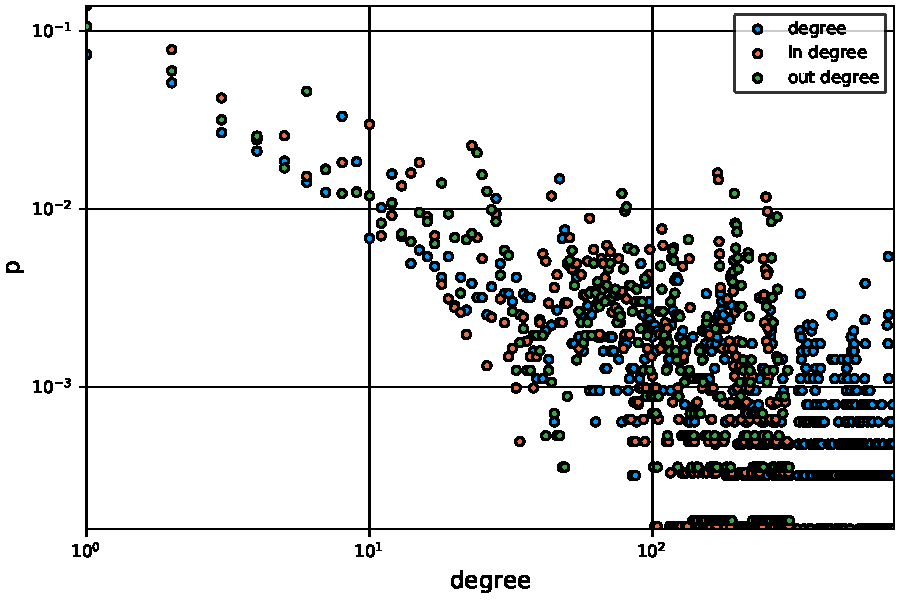
\includegraphics[width=0.45\textwidth]{../plots/degree}
  \caption{The in-degree, out-degree and degree distributions of the network.}
  \label{fig:dist}
\end{figure}

\begin{figure}
  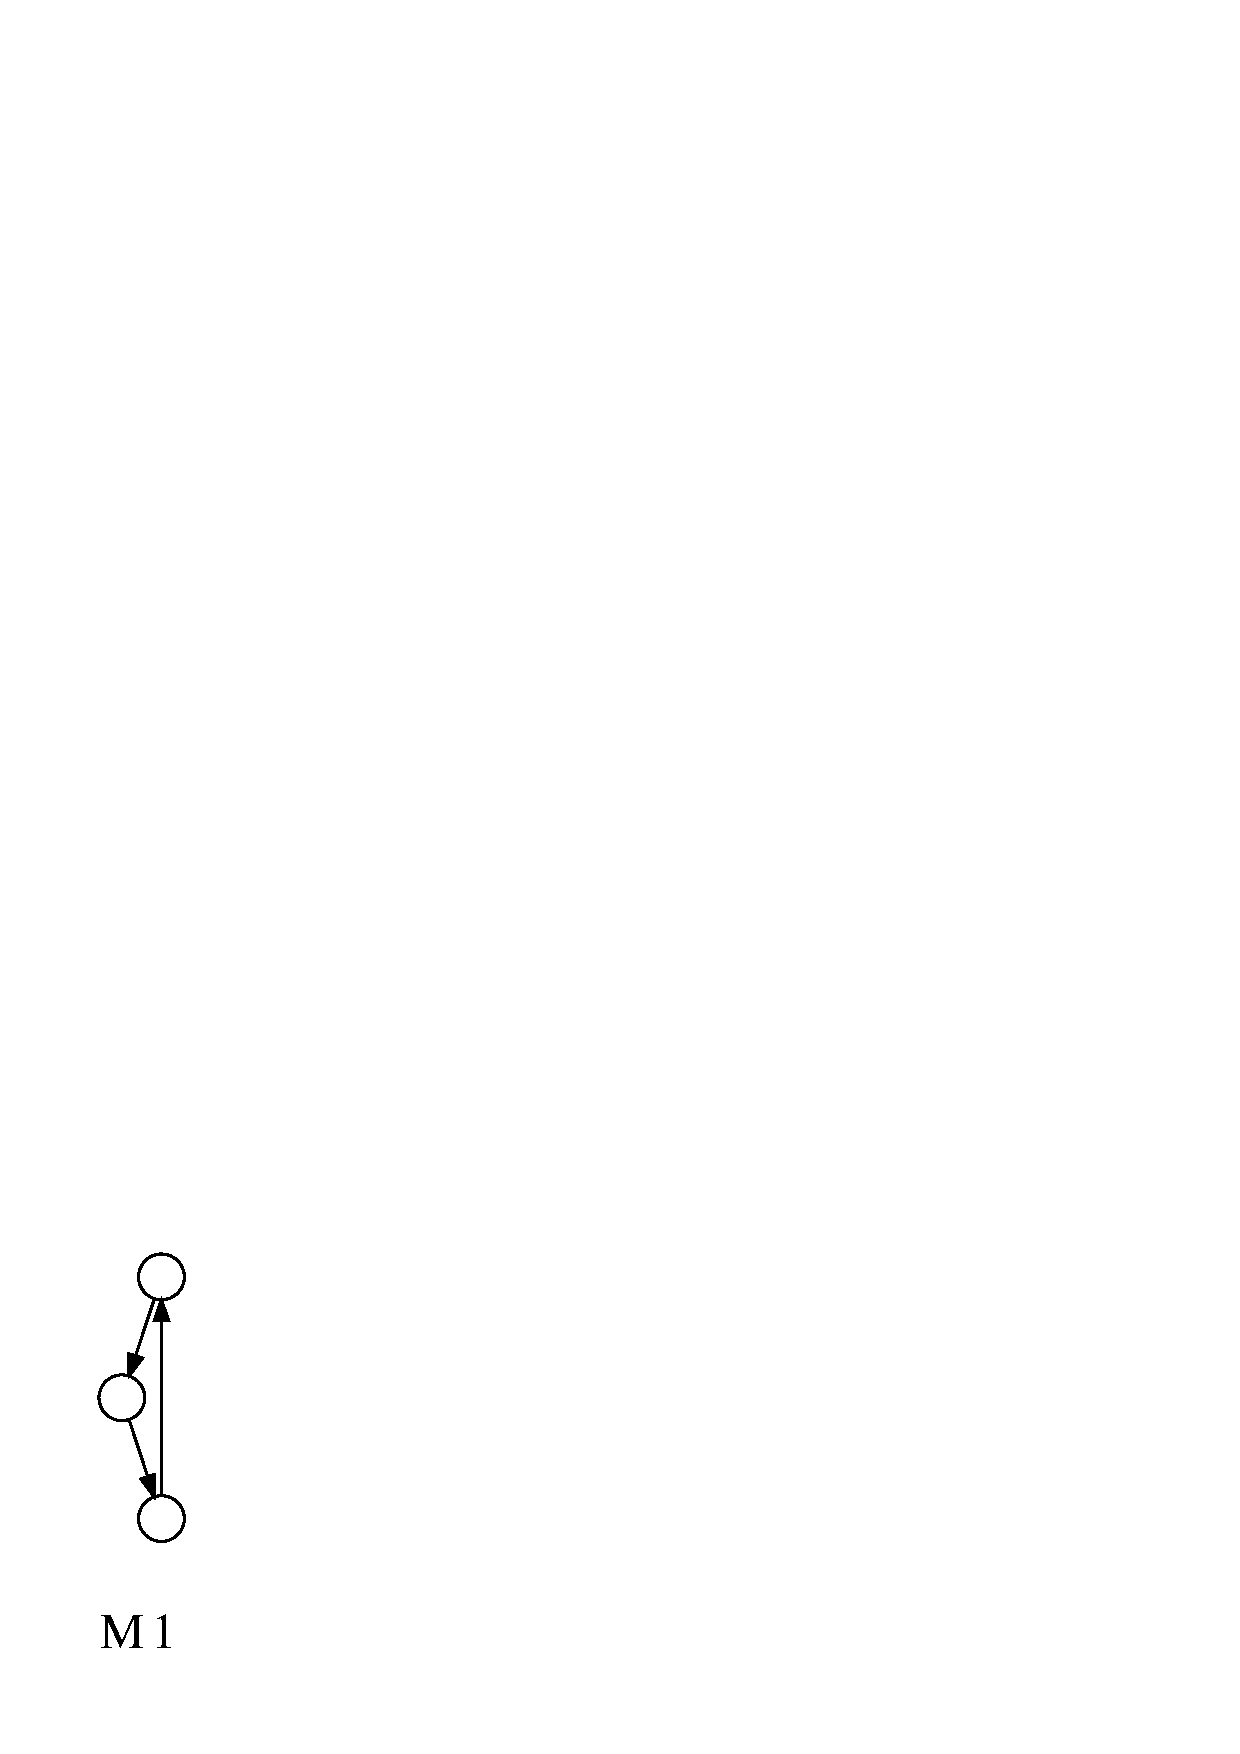
\includegraphics[width=0.03\textwidth]{M1-prc}
  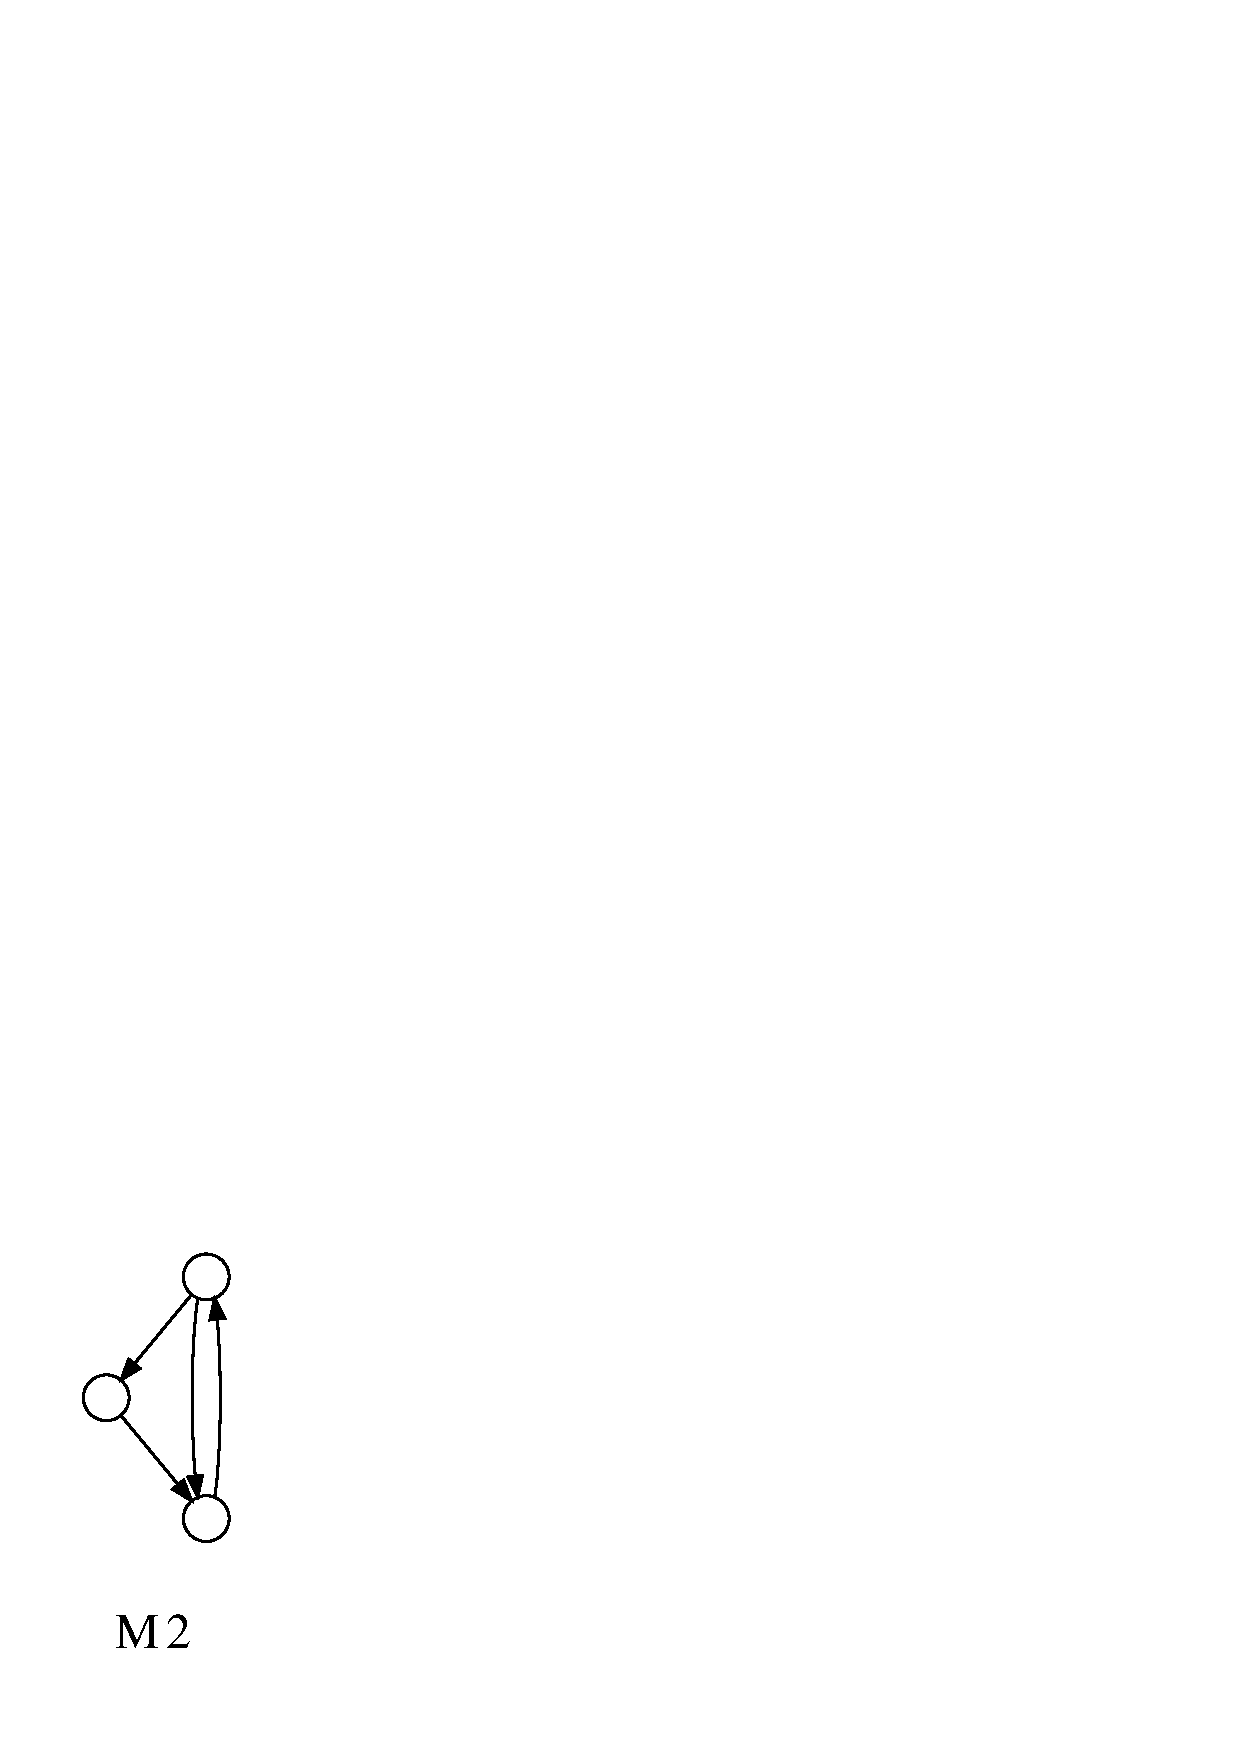
\includegraphics[width=0.03\textwidth]{M2-prc}
  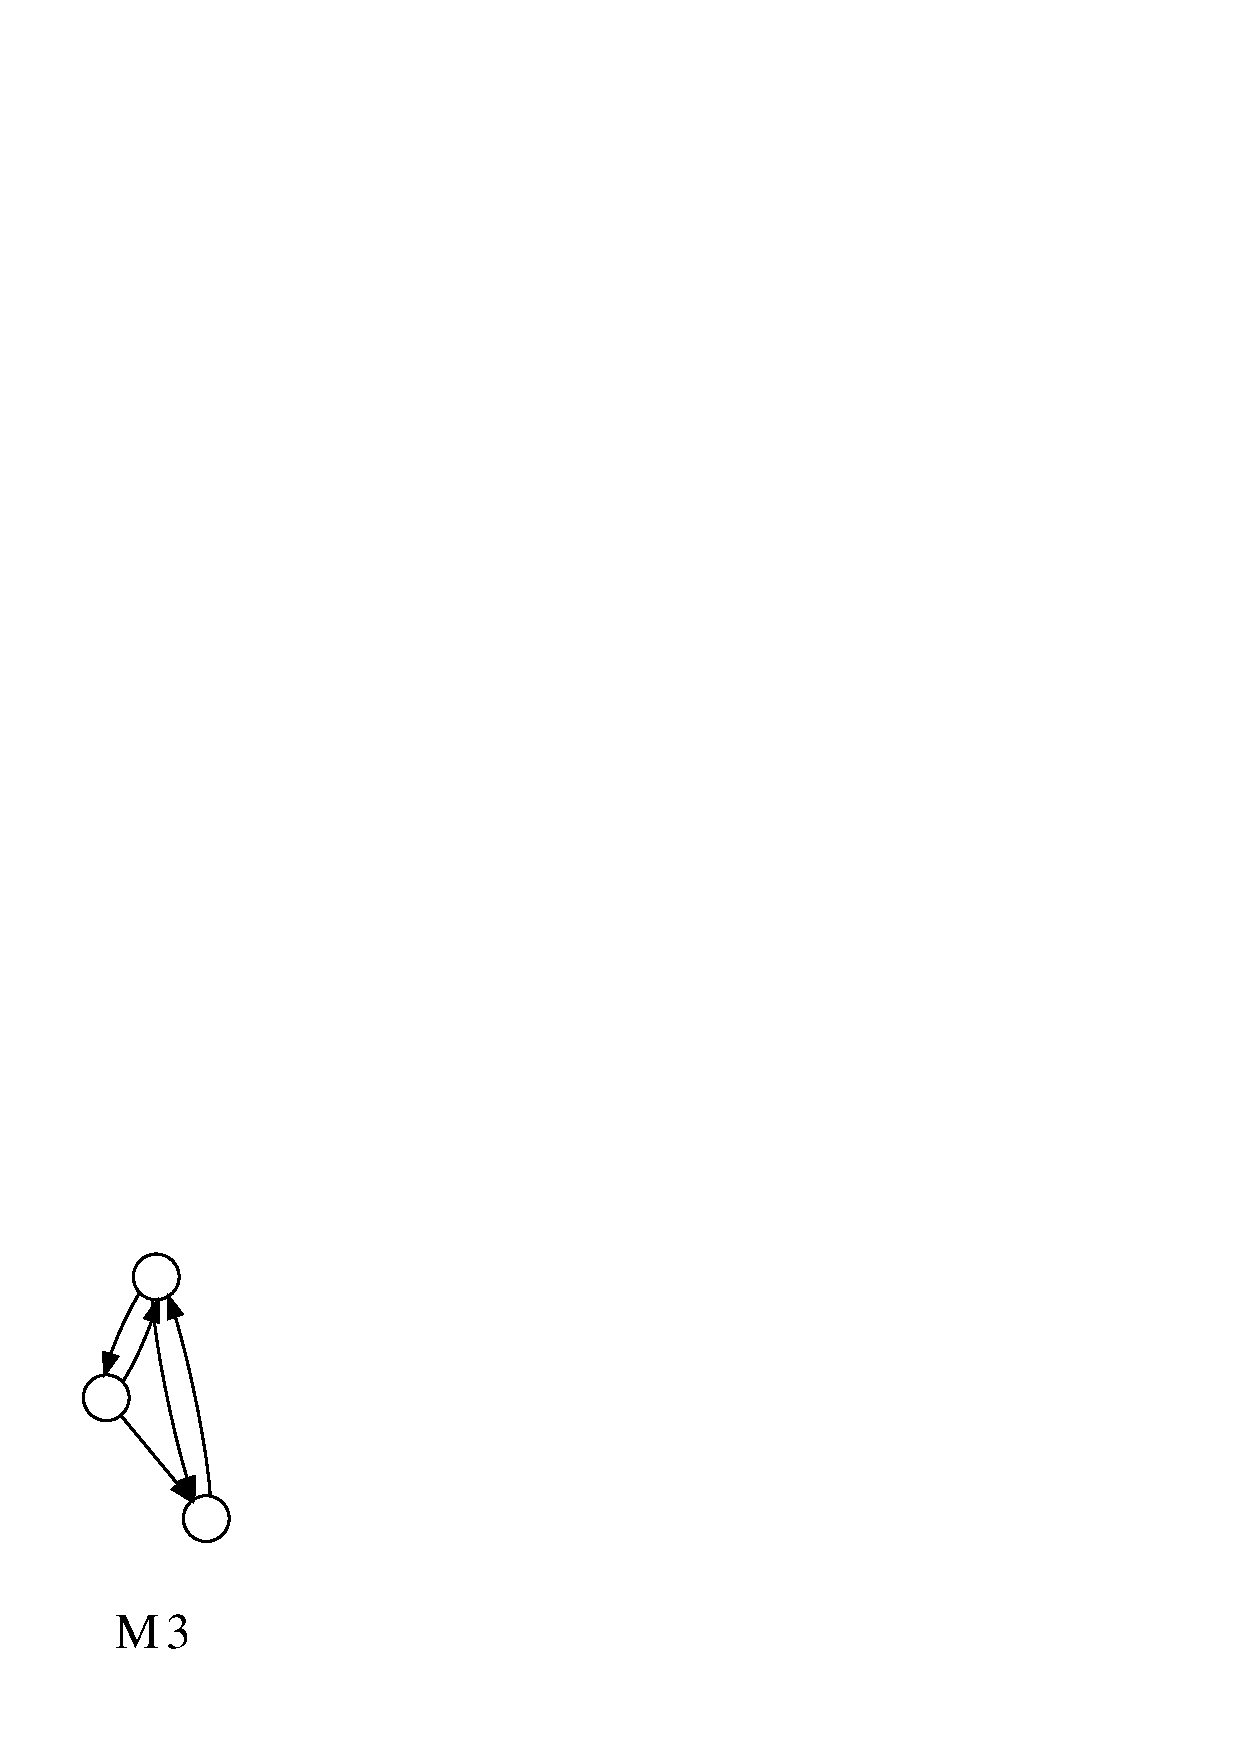
\includegraphics[width=0.03\textwidth]{M3-prc}
  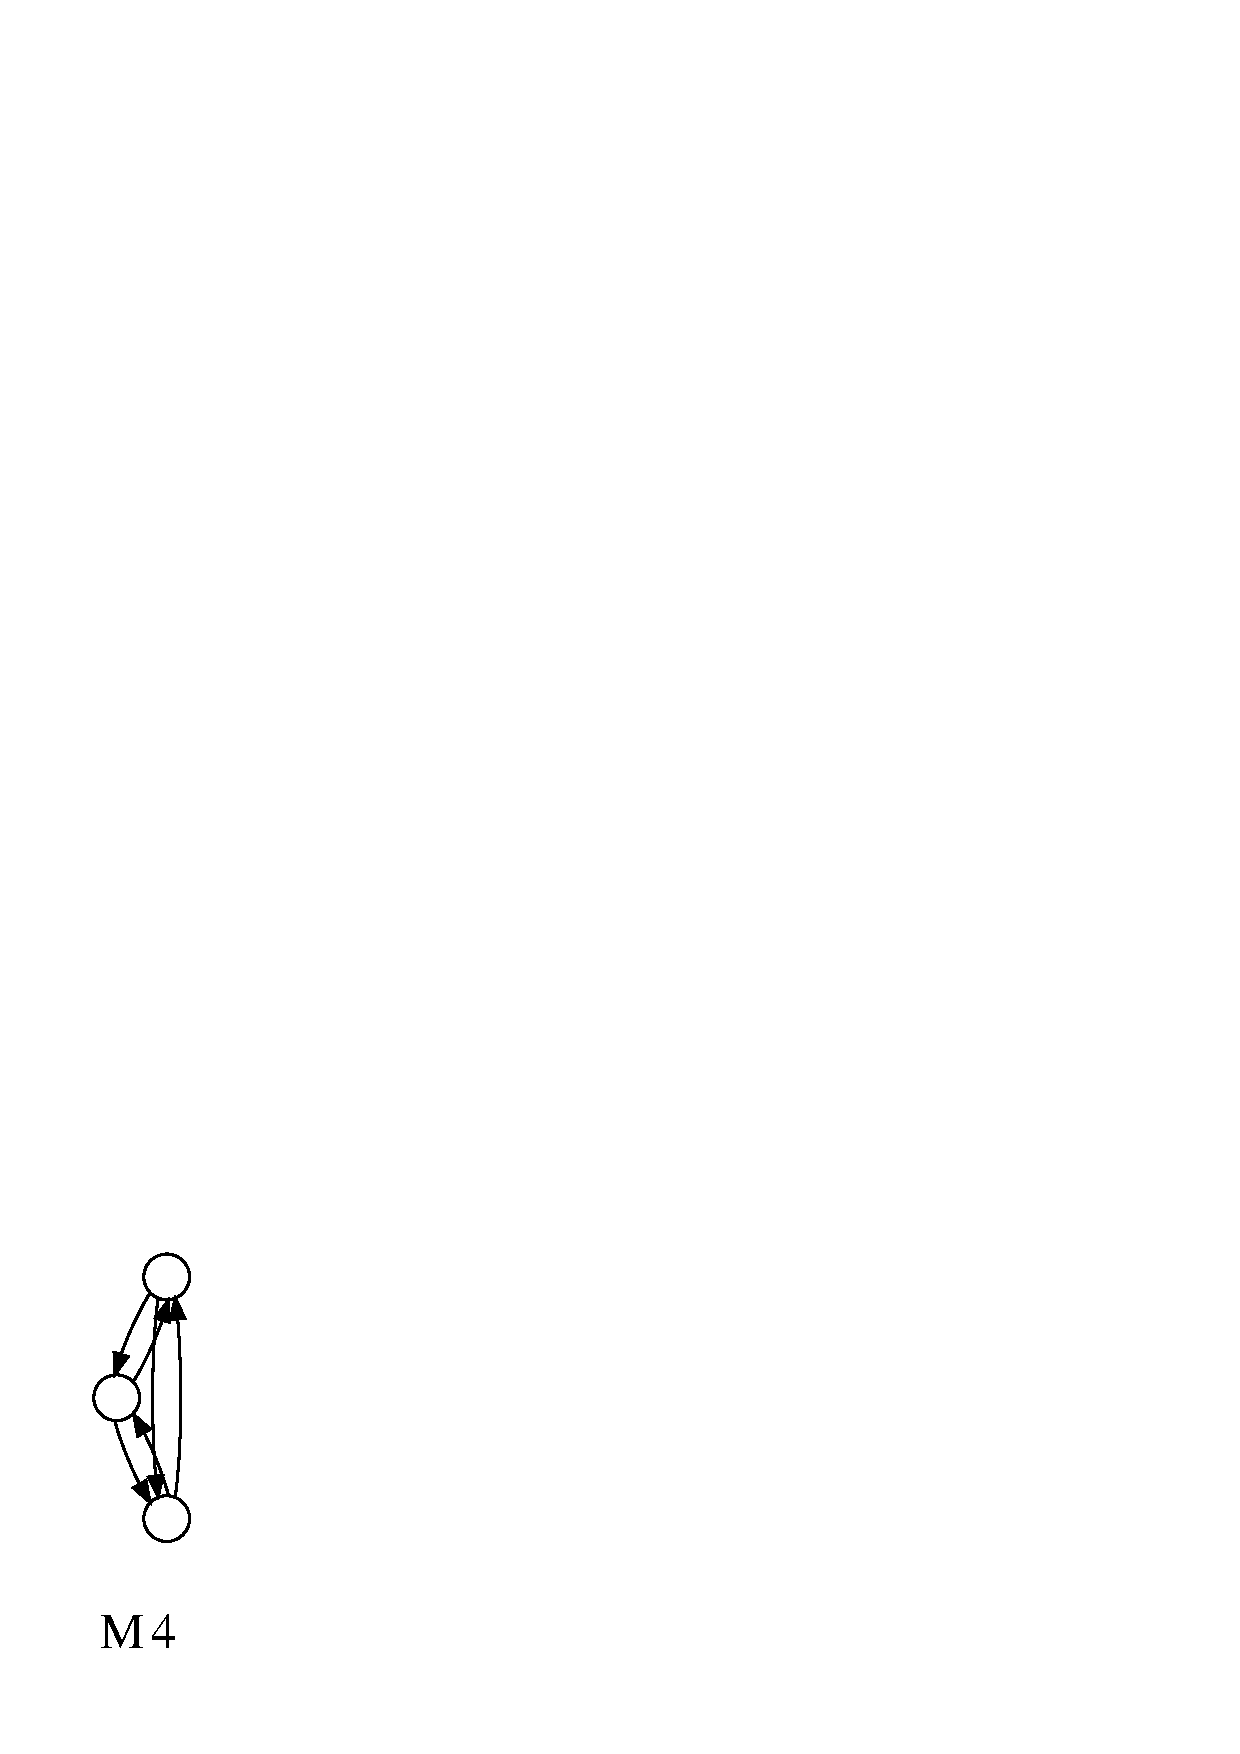
\includegraphics[width=0.03\textwidth]{M4-prc}
  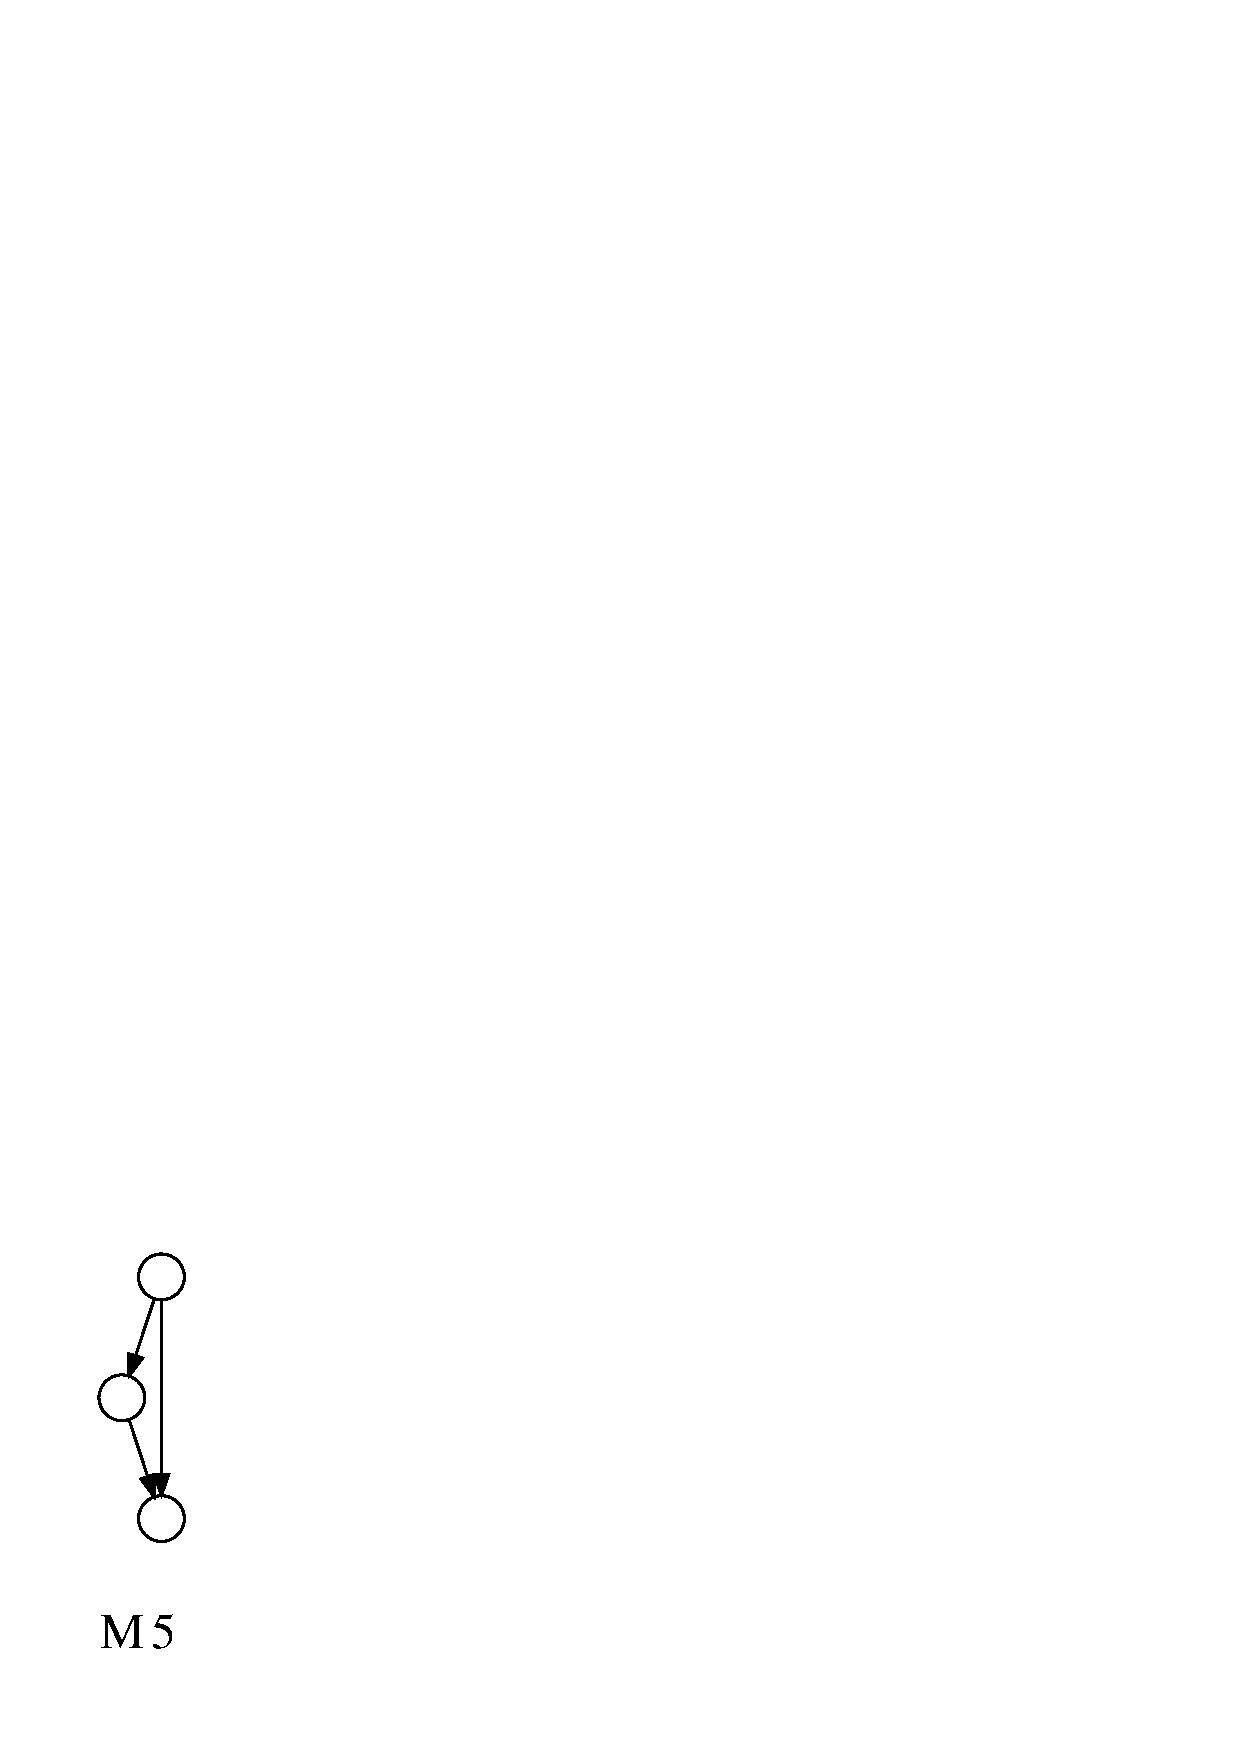
\includegraphics[width=0.03\textwidth]{M5-prc}
  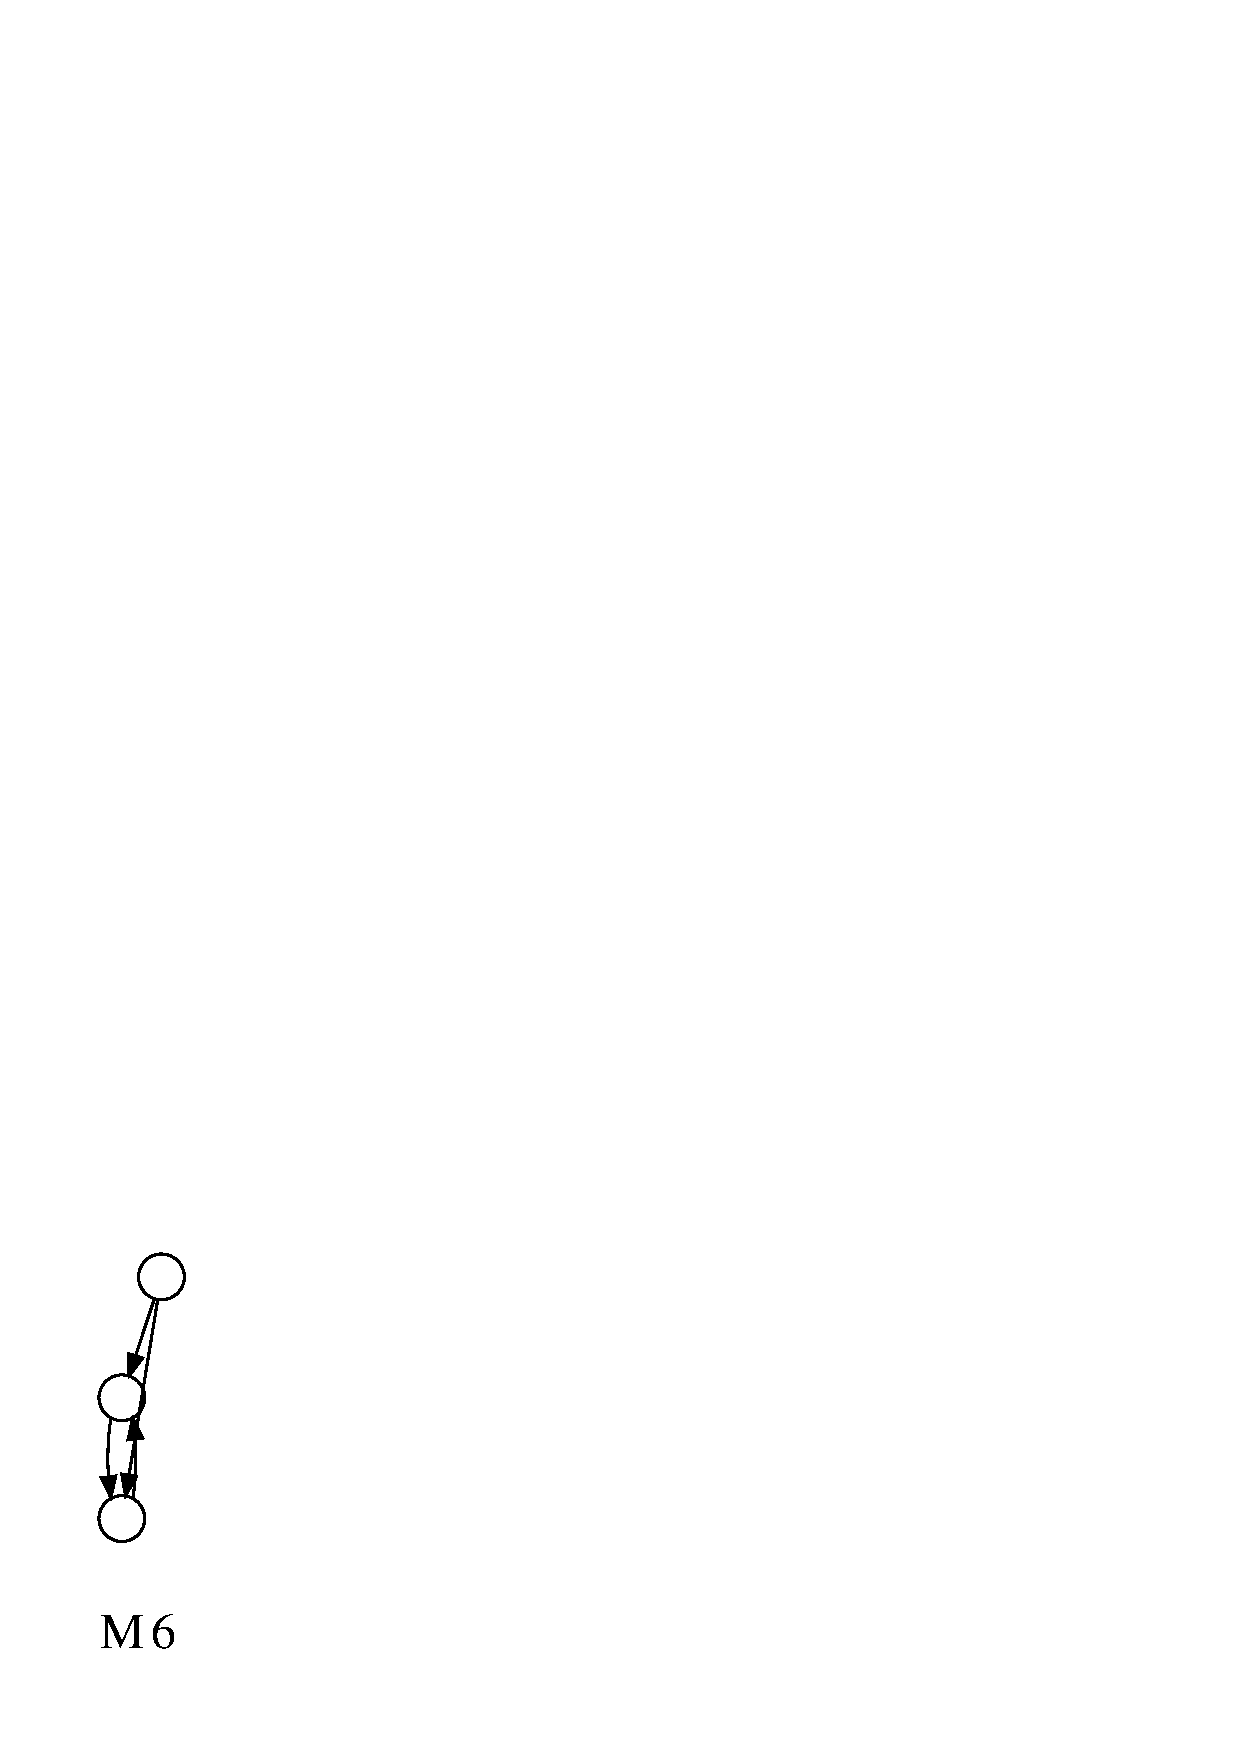
\includegraphics[width=0.03\textwidth]{M6-prc}
  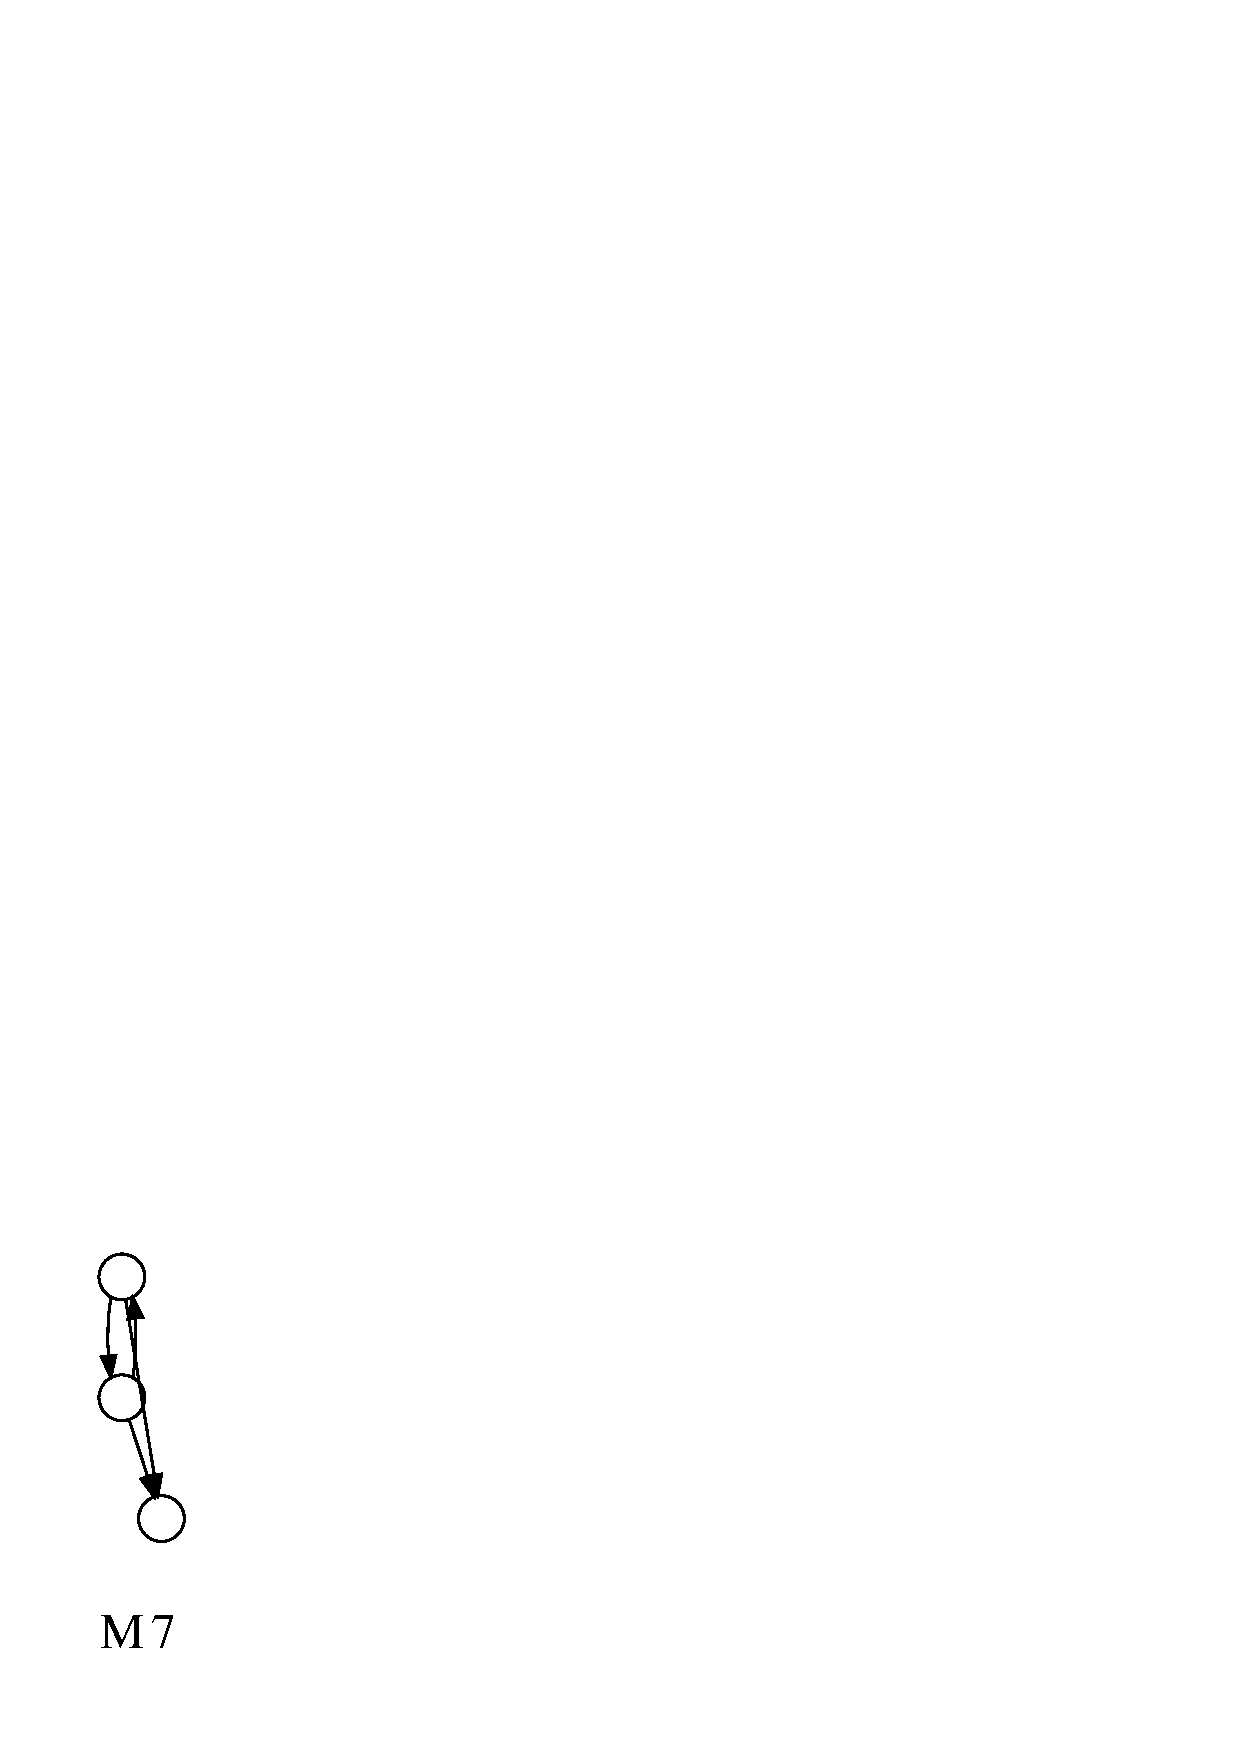
\includegraphics[width=0.03\textwidth]{M7-prc}
  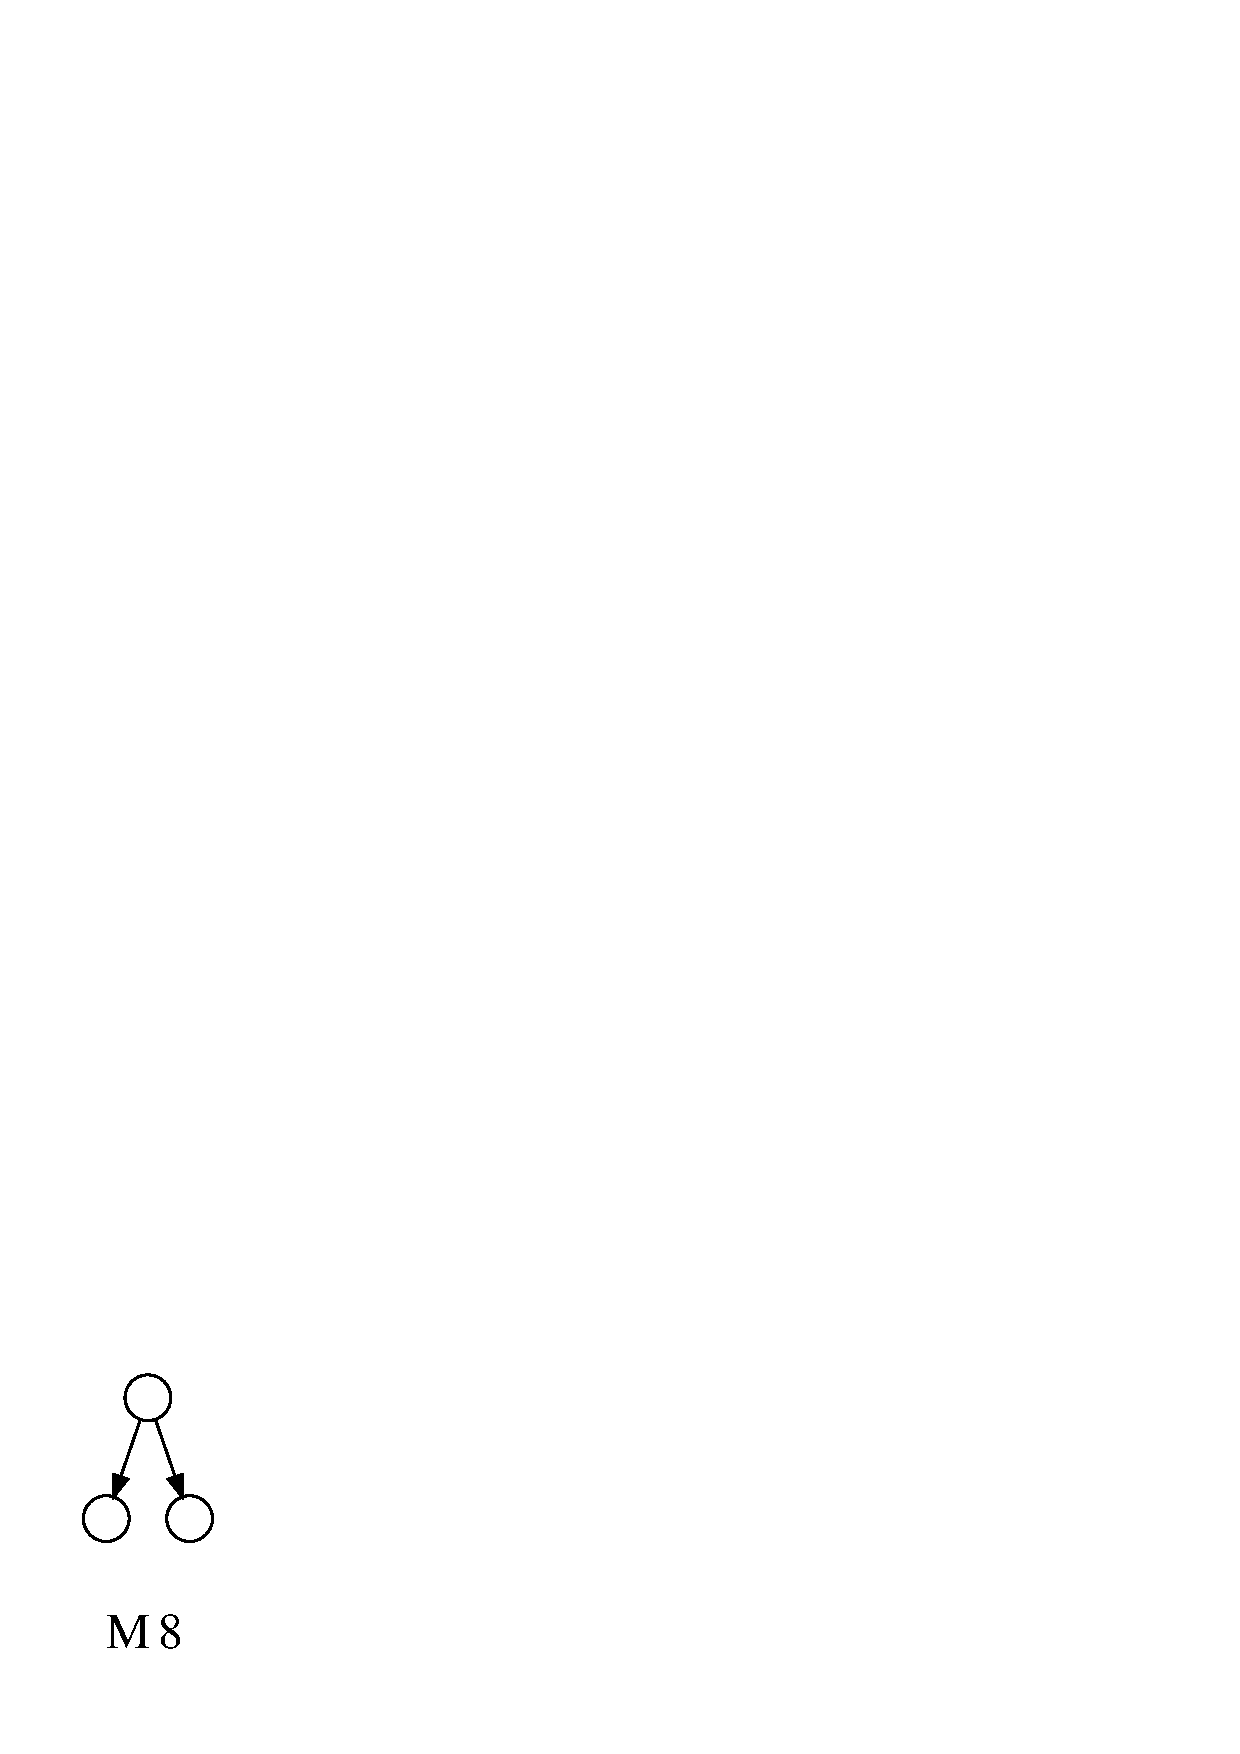
\includegraphics[width=0.03\textwidth]{M8-prc}
  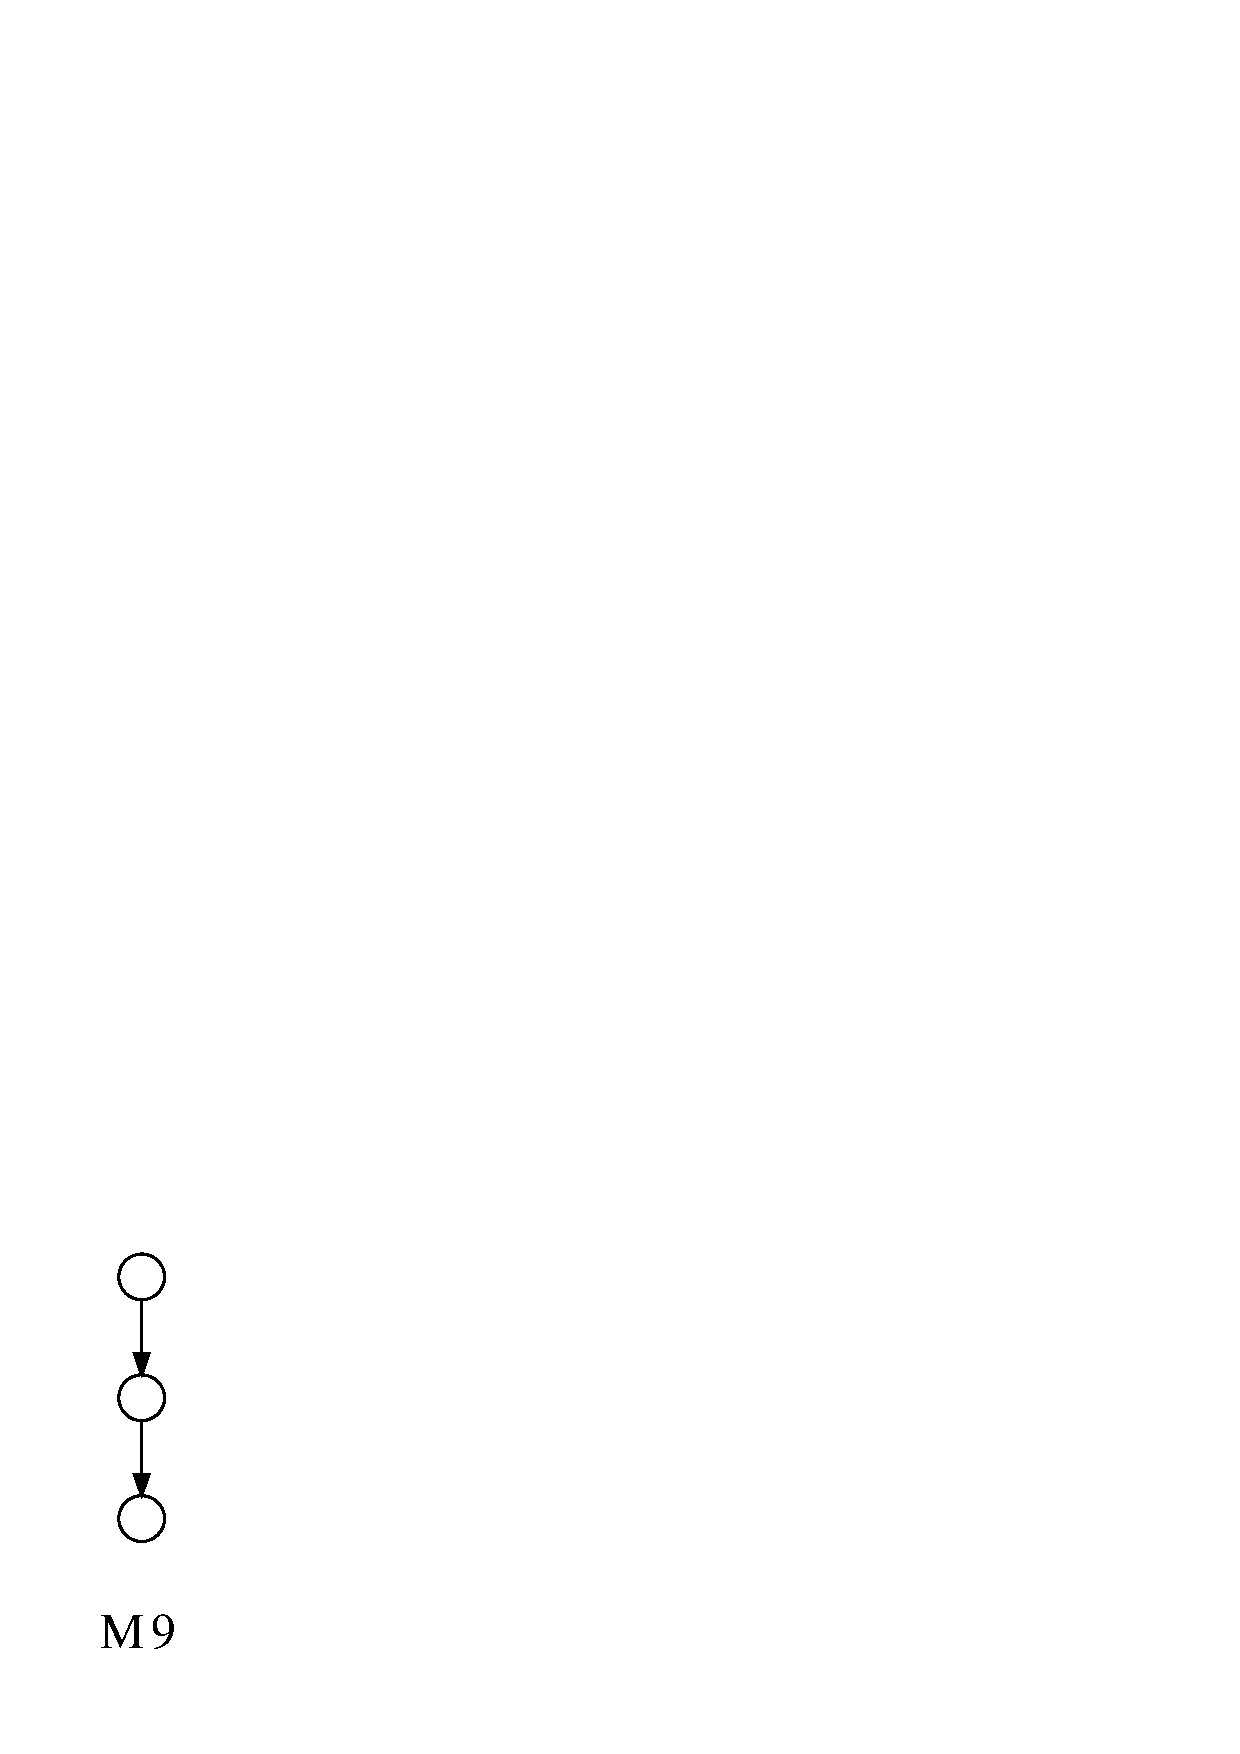
\includegraphics[width=0.03\textwidth]{M9-prc}
  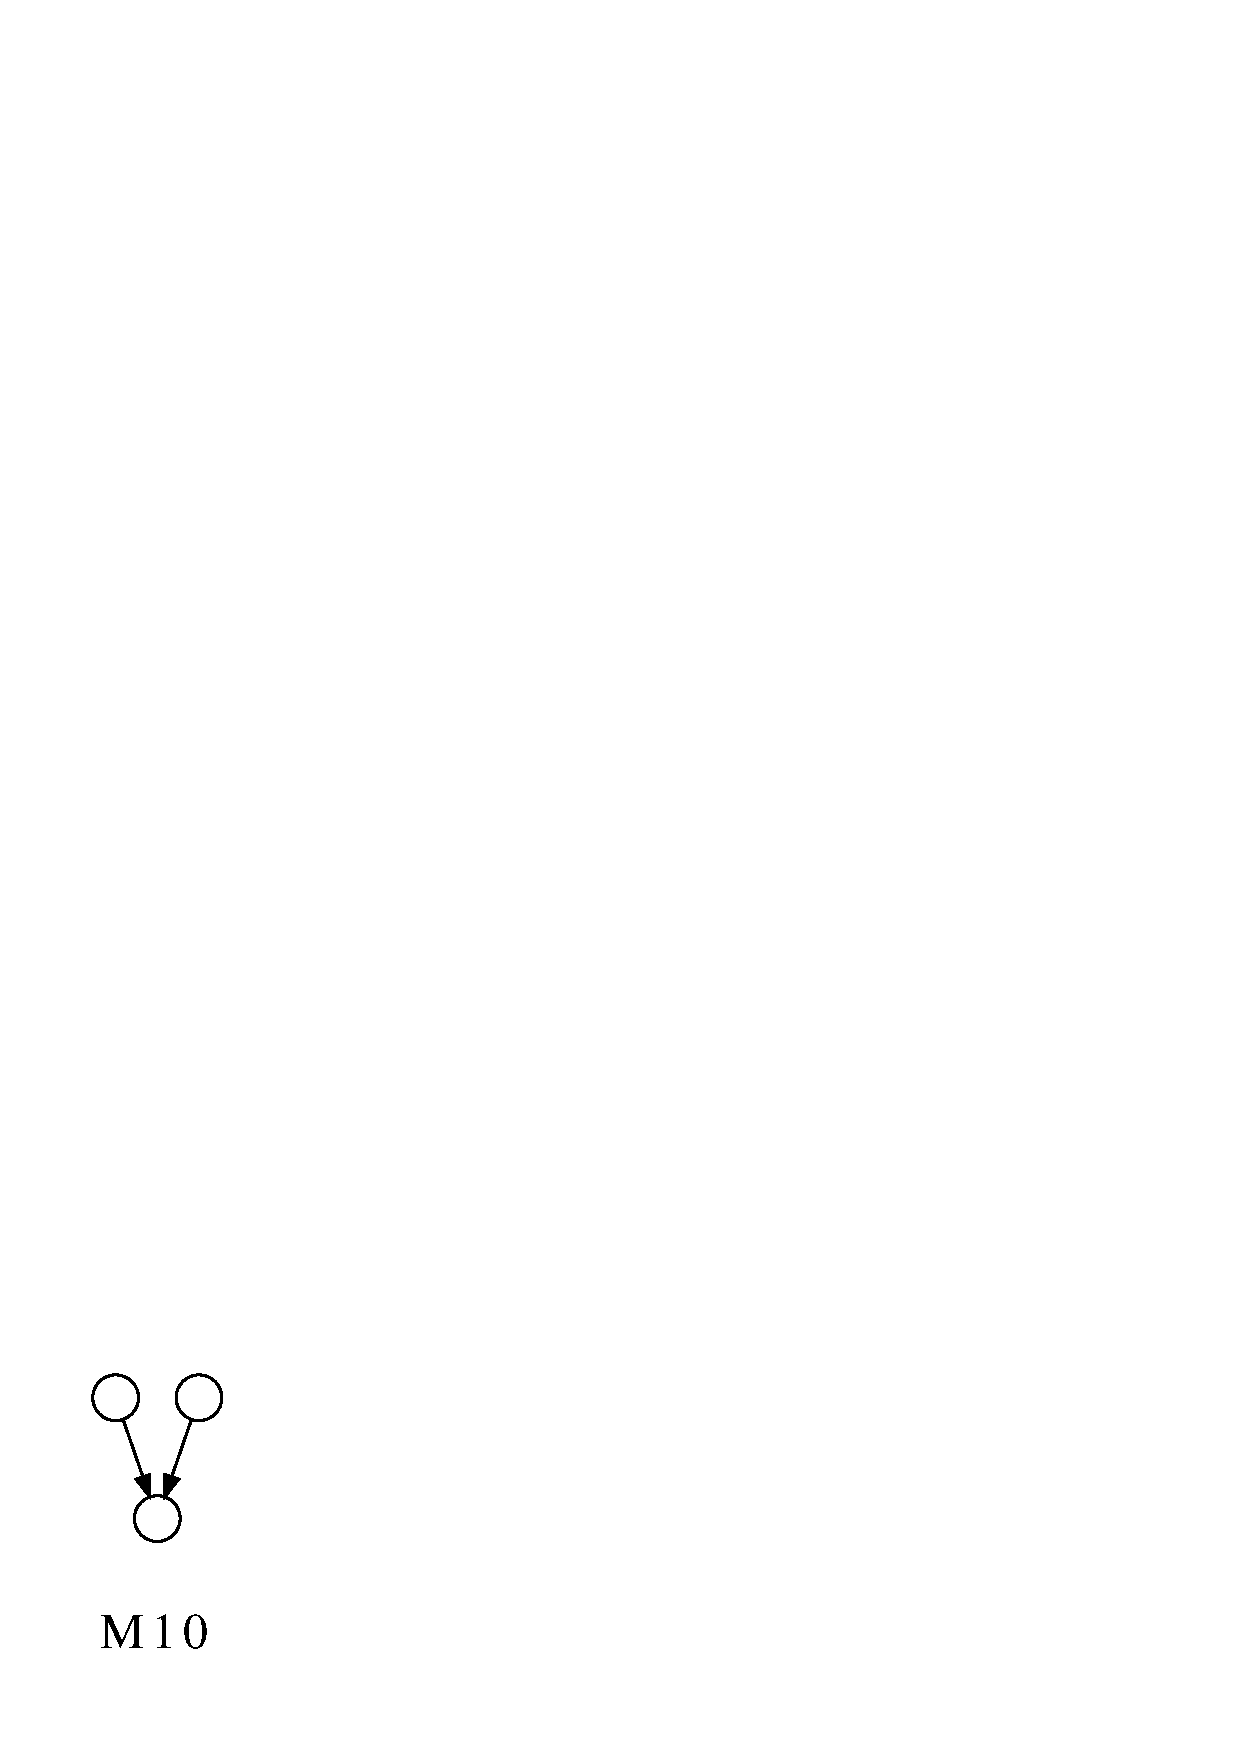
\includegraphics[width=0.03\textwidth]{M10-prc}
  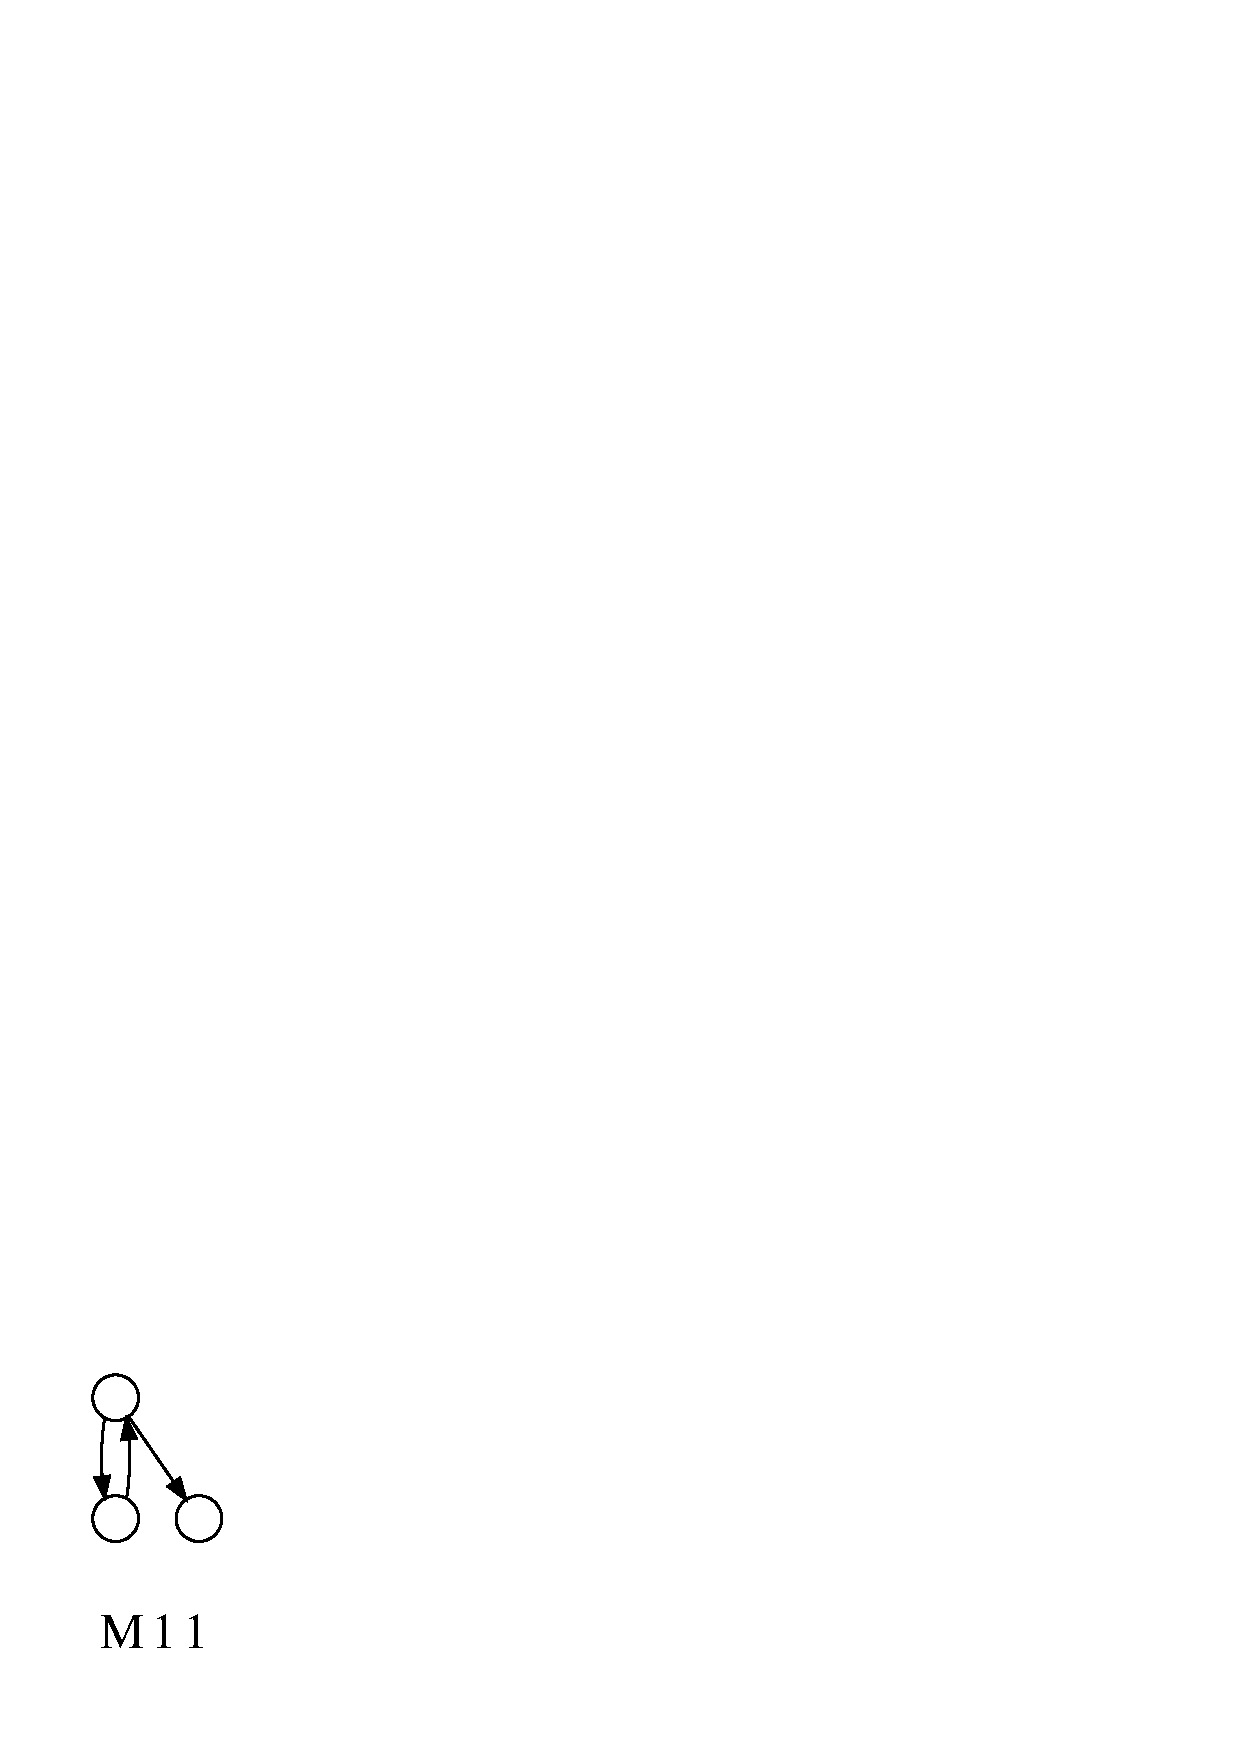
\includegraphics[width=0.03\textwidth]{M11-prc}
  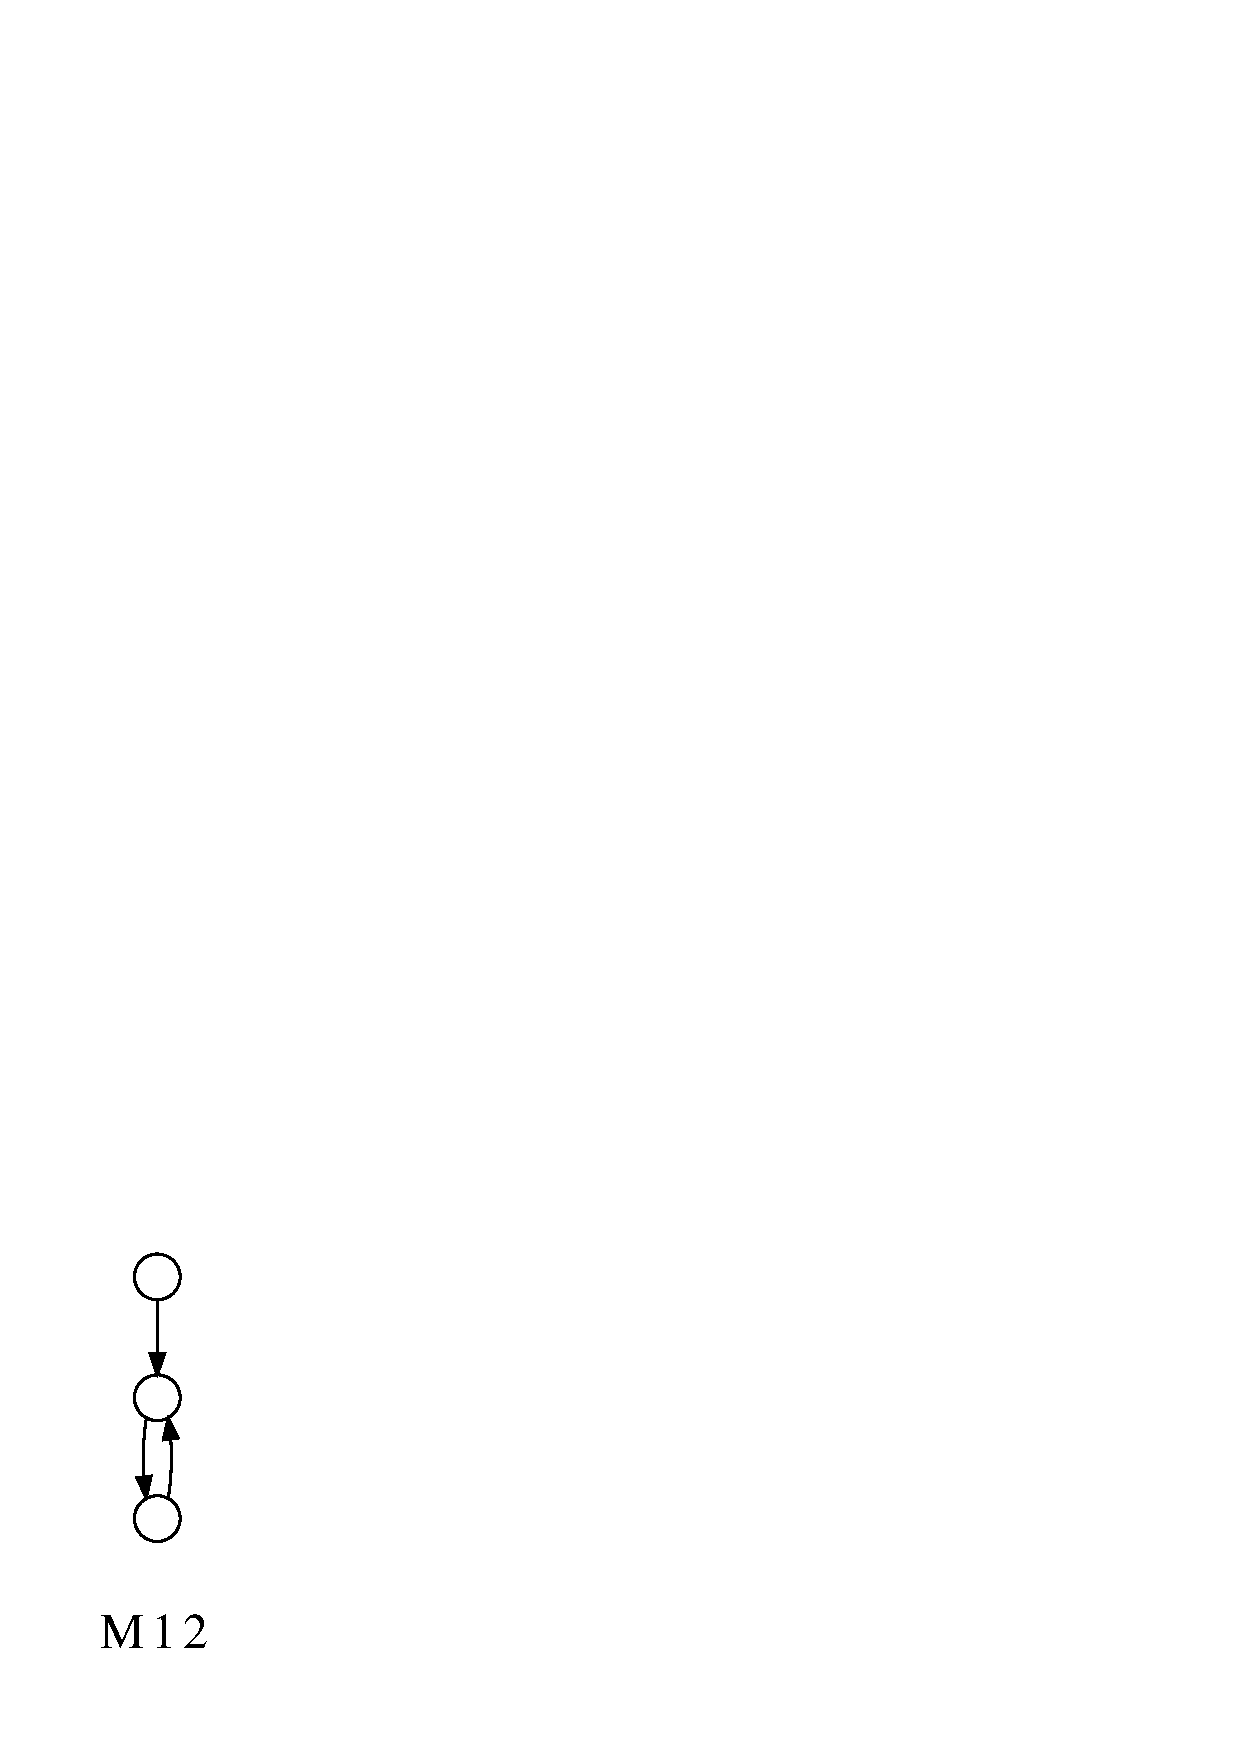
\includegraphics[width=0.03\textwidth]{M12-prc}
  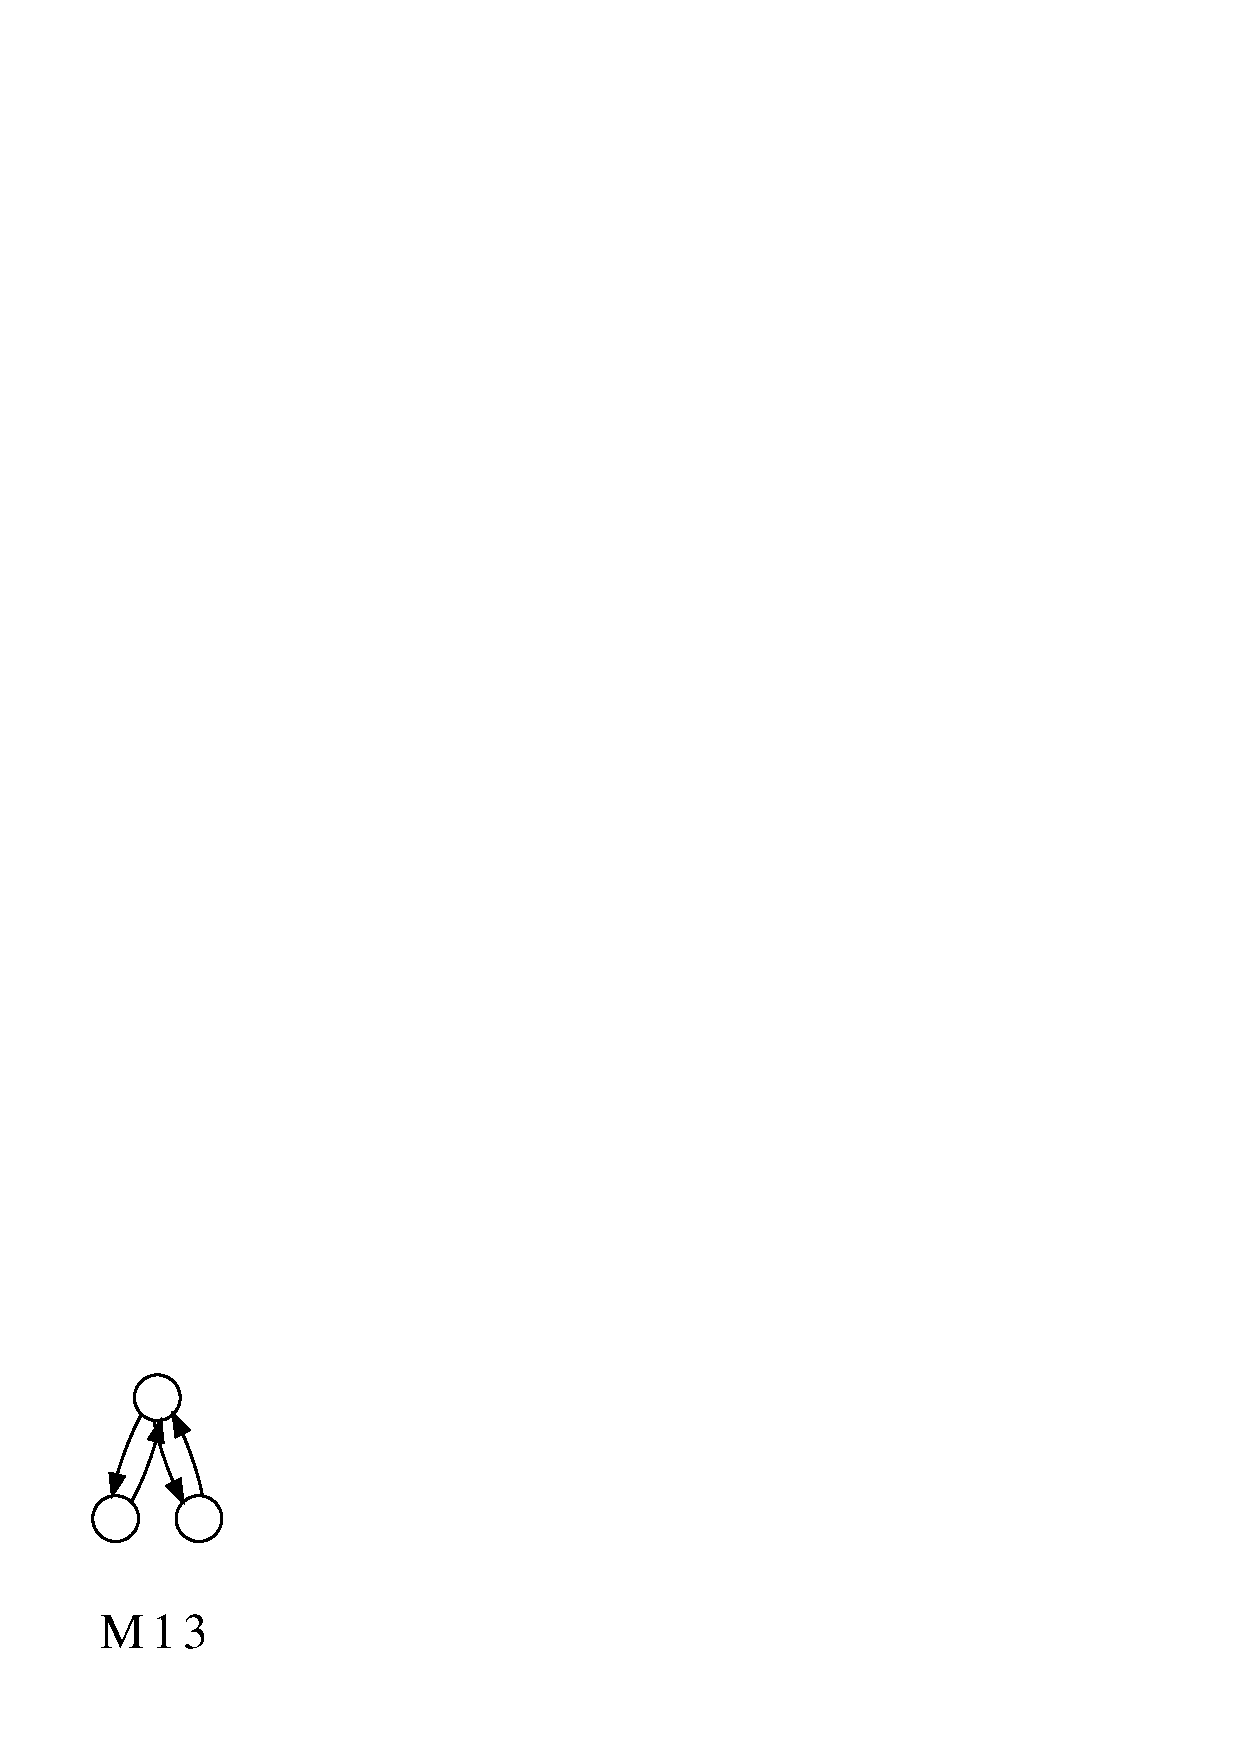
\includegraphics[width=0.03\textwidth]{M13-prc}
  \caption{All 13 directed three-node motifs.}
  \label{fig:motifs}
\end{figure}

\section{Authors contributions}
All the authors were involved in the preparation of the manuscript.
All the authors have read and approved the final manuscript.

\bibliographystyle{plain}
\bibliography{biblio}

\end{document}

% TEMPLATES FOR TABLES AND FIGURES

%\begin{table}
%\caption{Please write your table caption here}
%\label{tab:1}       % Give a unique label
%\begin{tabular}{lll}
%\hline\noalign{\smallskip}
%first & second & third  \\
%\noalign{\smallskip}\hline\noalign{\smallskip}
%number & number & number \\
%number & number & number \\
%\noalign{\smallskip}\hline
%\end{tabular}
%% Or use
%\vspace*{5cm}  % with the correct table height
%\end{table}

%% For one-column wide figures use
%\begin{figure}
%% Use the relevant command for your figure-insertion program
%% to insert the figure file.
%% For example, with the option graphics use
%\resizebox{0.75\textwidth}{!}{%
%  
\includegraphics{leer.eps}
%}
%% If not, use
%%\vspace{5cm}       % Give the correct figure height in cm
%\caption{Please write your figure caption here}
%\label{fig:1}       % Give a unique label
%\end{figure}

%% For two-column wide figures use
%\begin{figure*}
%% Use the relevant command for your figure-insertion program
%% to insert the figure file. See example above.
%% If not, use
%\vspace*{5cm}       % Give the correct figure height in cm
%\caption{Please write your figure caption here}
%\label{fig:2}       % Give a unique label
%\end{figure*}
